%!TEX root = ../main.tex

\setchapterpreamble[ul][0.6\textwidth]{%
    \dictum[Douglas Adams, \textit{The Hitchhiker’s Guide to the Galaxy}]{%
        \enquote{\foreignlanguage{english}{He attacked everything in life with a mixture of extraordinary genius and naive incompetence and it was often difficult to tell which was which.}}
    }
    \vspace*{2\baselineskip}
}
\chapter{Einleitung} % (fold)
\label{cha:einleitung}

Ein Polymer, oder auch Makromolekül, ist ein Molekül, welches sich aus vielen kleineren, sich wiederholenden Molekülen, sogenannten Monomeren, zusammensetzt.
Besteht ein Polymer aus nur einer Monomer-Art, dann spricht man von einem Homopolymer, sonst von einem Heteropolymer oder auch Copolymer.
Typischerweise besteht ein Polymer aus einer langen Kette von aneinanderhängenden Monomeren, es existieren aber auch weitere Konfigurationen, zum Beispiel stern- oder ringförmige Anordnungen.

Copolymere lassen sich anhand der Anordnung der Monomere weiter klassifizieren.
Bilden die verschiedenen Monomer-Gattungen homogene, zusammenhängende Gruppen, welche wiederum durch aneinanderreihen das Copolymer bilden, dann nennen wir dies ein Blockcopolymer, vergleiche \cref{fig:konfig}.

Es existieren unüberschaubar viele solcher Konfigurationen von Polymeren, und insbesondere Blockcopolymeren, weswegen man häufig auf das Studium vergleichsweise simpler Anordnungen zurückgreift.
Als besonders beliebt hat sich der Fall des kettenförmigen Blockcopolymers mit zwei Monomer-Typen, der Einfachheit halber A und B genannt, herausgestellt.
Diese Konfiguration wird auch als AB-Diblockcopolymer bezeichnet.

\begin{figure}[tb]
    \centering
    \begin{subfigure}[b]{\textwidth}
        \centering
        \includestandalone[width=0.8\textwidth]{tikz/einleitung/fig1}
    \end{subfigure}
    \\[1em]
    \begin{subfigure}[b]{\textwidth}
        \centering
        \includestandalone[width=0.8\textwidth]{tikz/einleitung/fig2}
    \end{subfigure}
    \\[1em]
    \begin{subfigure}[b]{\textwidth}
        \centering
        \includestandalone[width=0.8\textwidth]{tikz/einleitung/fig3}
    \end{subfigure}
    \caption[Skizzenhafte Darstellung verschiedener Polymerarten]{%
        Skizzenhafte Darstellung verschiedener Polymerarten.
        Von oben nach unten: Homopolymer, ein AB-Diblockcopolymer und ein sogenanntes statistisches AB-Copolymer, bei dem die beiden Monomer-Arten zufällig verteilt sind.
    }
    \label{fig:konfig}
\end{figure}

Von großem Interesse ist das Verhalten von Polymerschmelzen (\foreign{engl.}{polymer melt}), das heißt, des flüssigen Aggregatzustands eines Polymers, sowie das Verhalten von Gemischen verschiedener polymerer Stoffe.
So neigen die Gemische vieler Paare von Homopolymeren zu makroskopischer Phasenseparation, wie man es zum Beispiel von Öl und Essig kennt.
Eine ähnliche Tendenz findet man auch bei den Polymerschmelzen von Blockcopolymeren, hierbei kann aufgrund der Verbindung der verschiedenen Monomer-Blöcke aber keine makroskopische Phasenseparation auftreten, stattdessen kommt es zu einer periodischen, mikroskopischen Separation.
\cref{fig:anordnungen} zeigt einige mögliche Anordnungen, die bei Diblockcopolymeren tatsächlich experimentell beobachtet wurden.

\begin{figure}[tb]
    \centering
    \begin{subfigure}[b]{0.18\textwidth}
        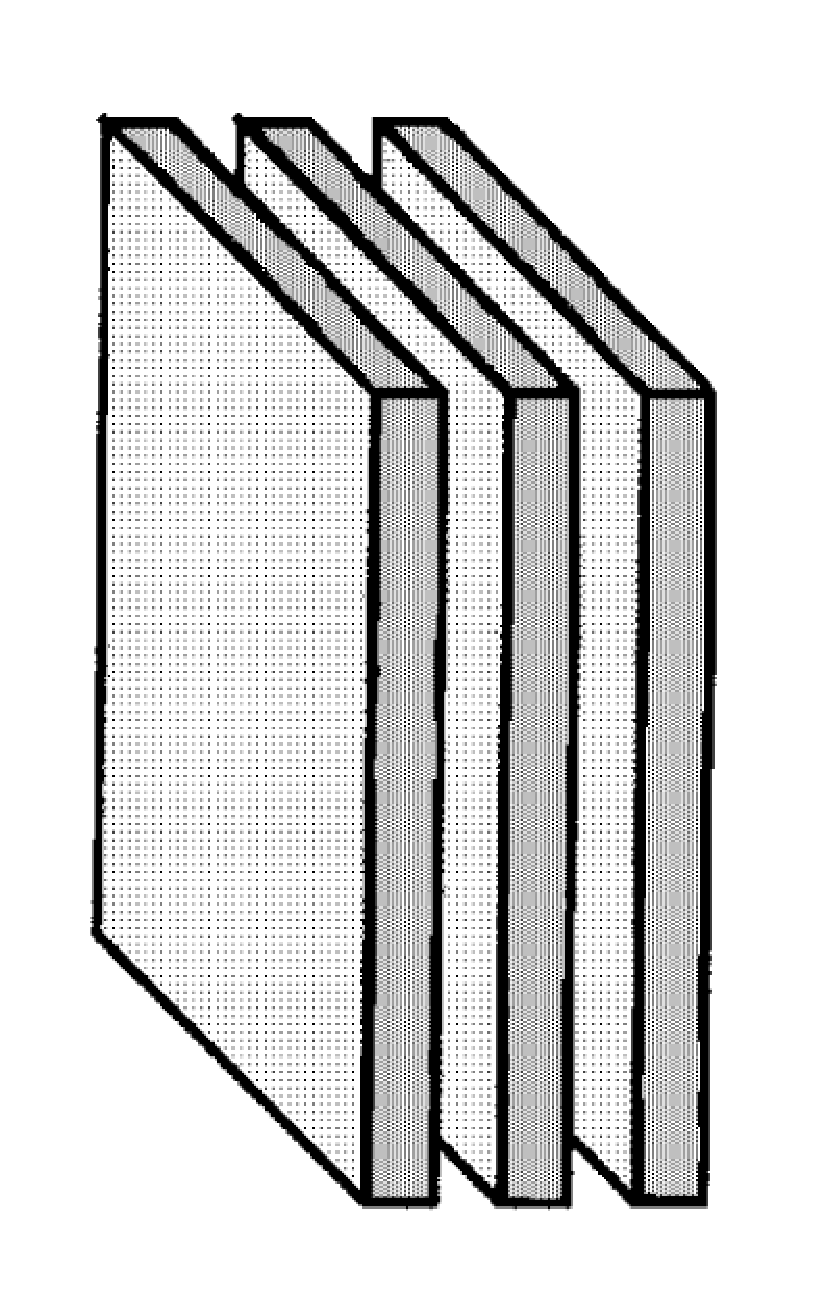
\includegraphics[width=\textwidth]{figures/einleitung/fig1}
    \end{subfigure}
    \begin{subfigure}[b]{0.18\textwidth}
        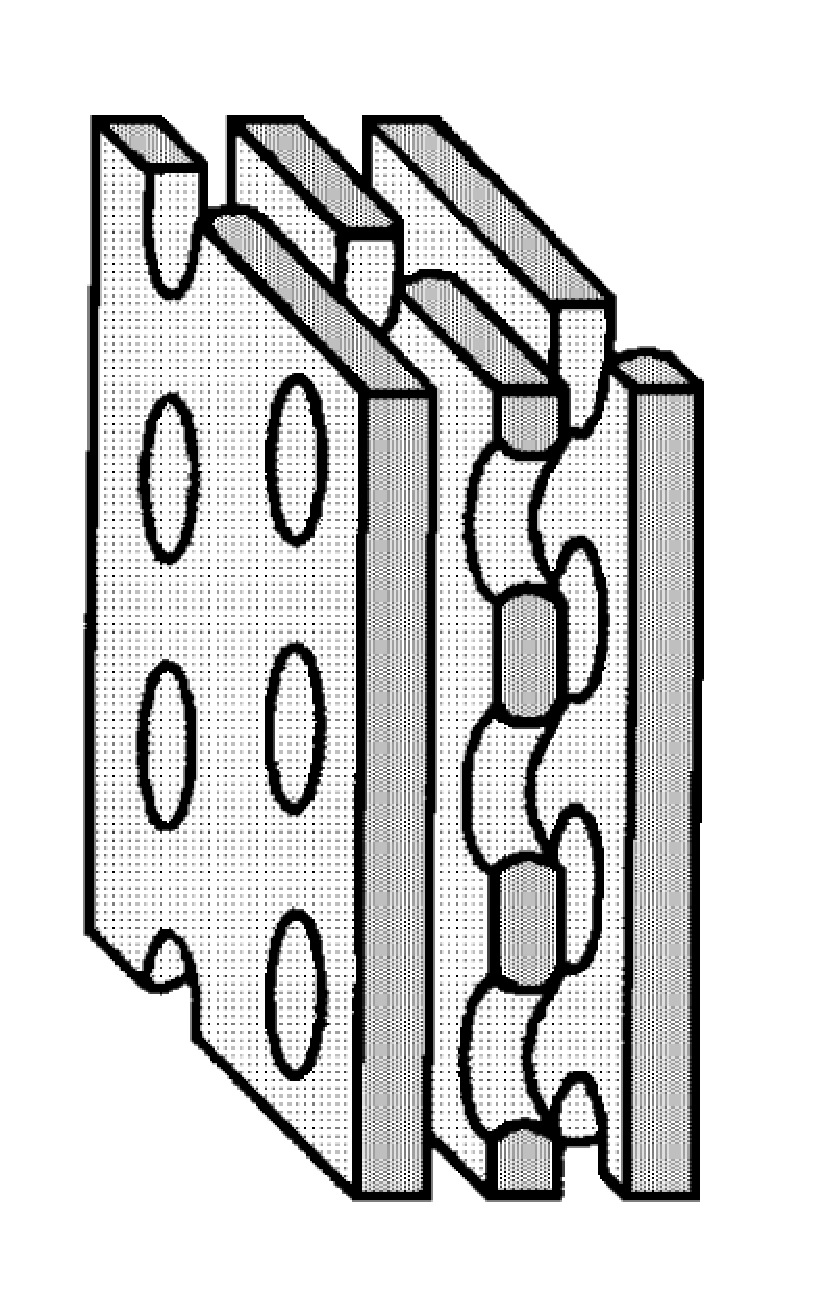
\includegraphics[width=\textwidth]{figures/einleitung/fig2}
    \end{subfigure}
    \begin{subfigure}[b]{0.18\textwidth}
        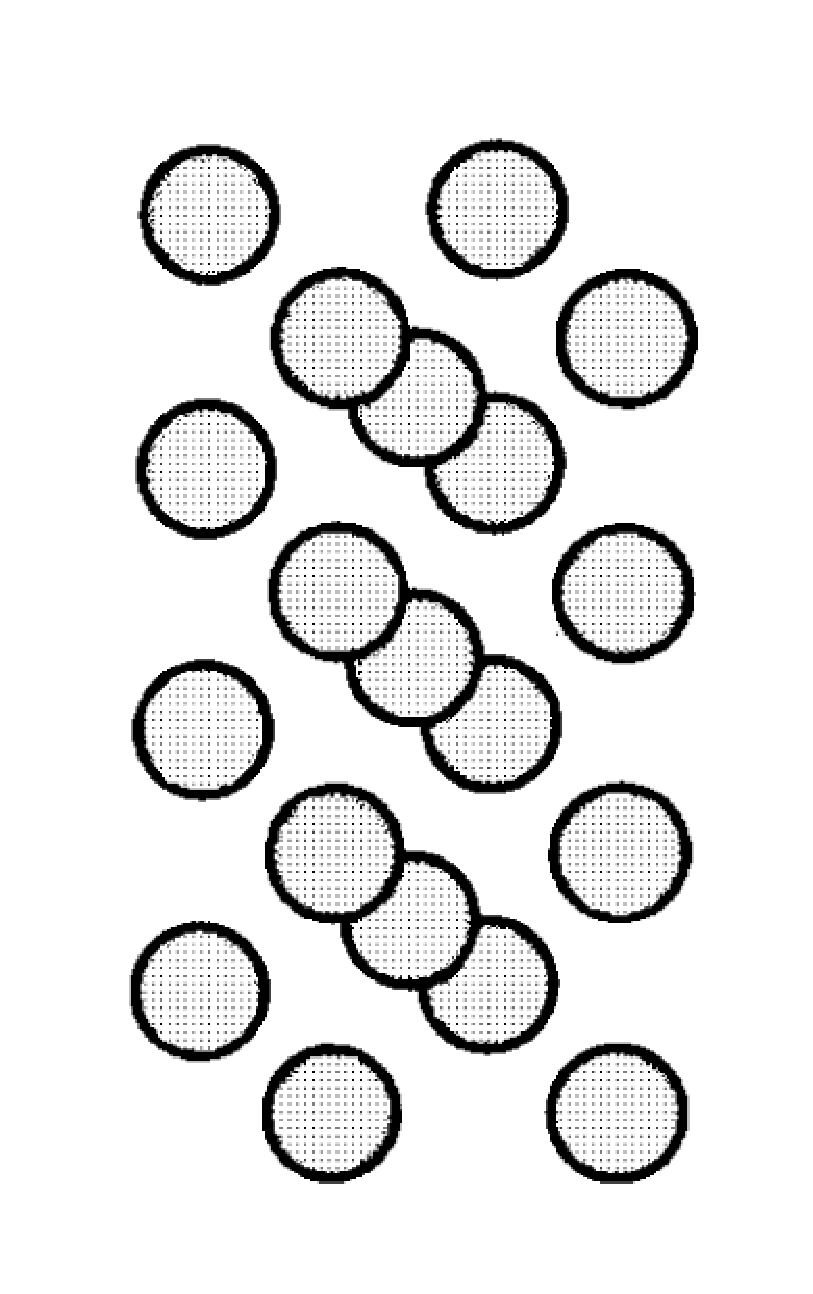
\includegraphics[width=\textwidth]{figures/einleitung/fig3}
    \end{subfigure}
    \begin{subfigure}[b]{0.18\textwidth}
        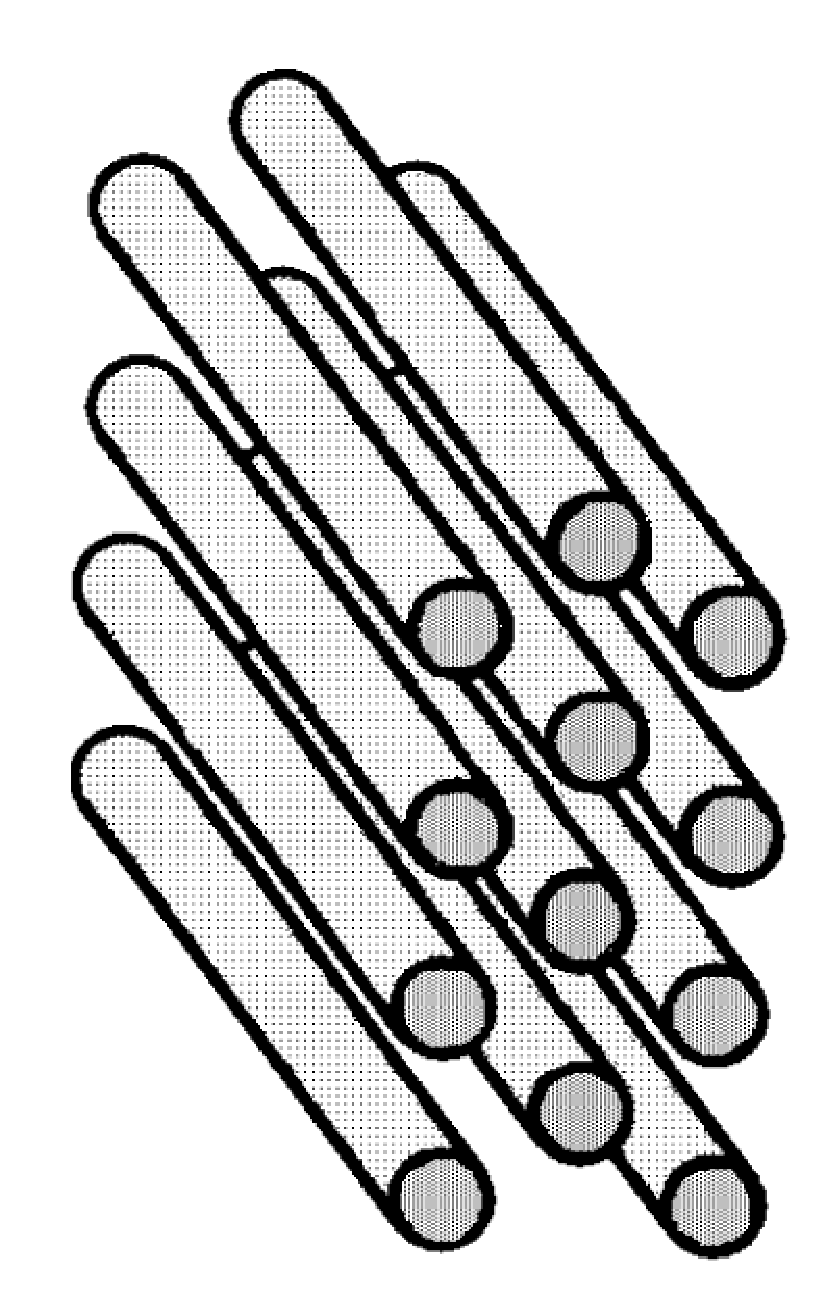
\includegraphics[width=\textwidth]{figures/einleitung/fig4}
    \end{subfigure}
    \begin{subfigure}[b]{0.18\textwidth}
        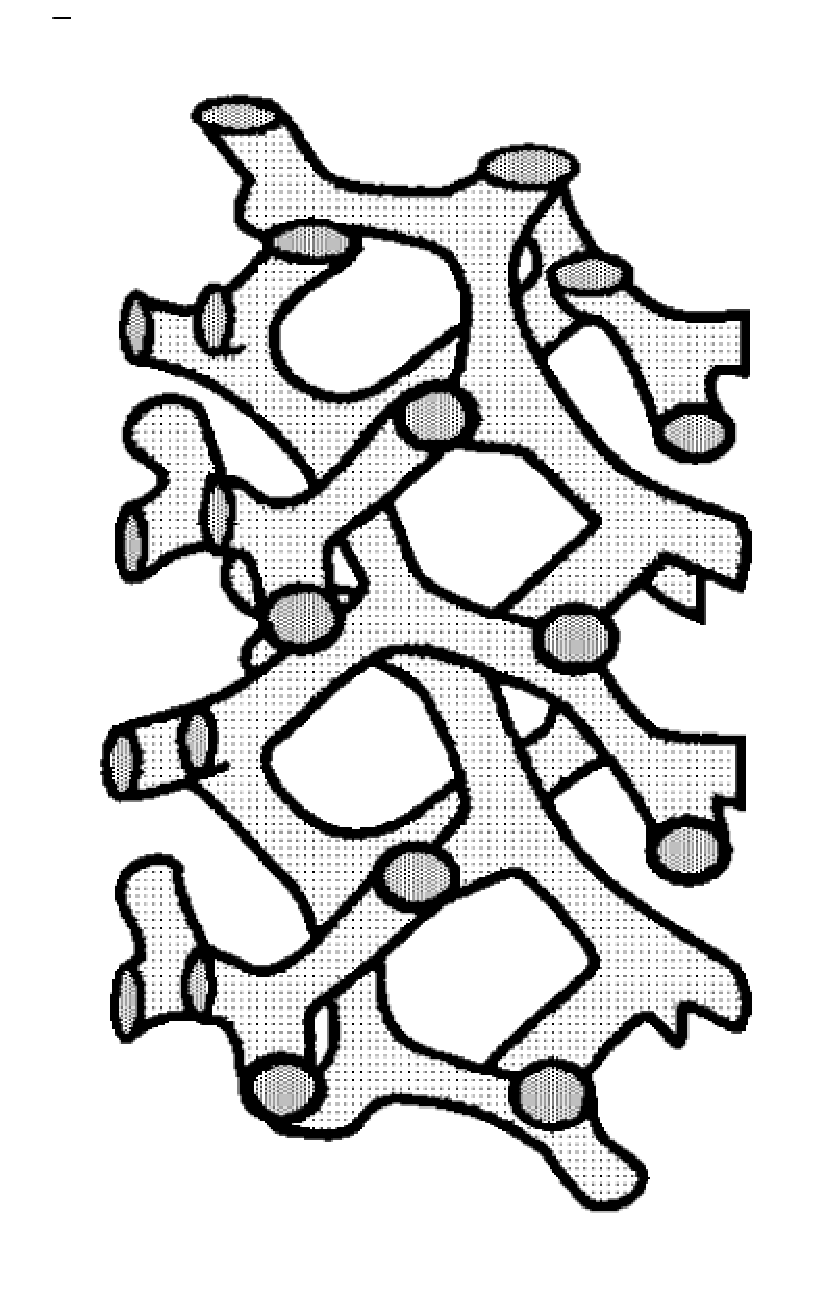
\includegraphics[width=\textwidth]{figures/einleitung/fig5}
    \end{subfigure}
    \caption[Verschiedene Phasen bei Diblockcopolymeren]{%
        Verschiedene Phasen bei Diblockcopolymeren, welche experimentell beobachtet wurden, wobei hierbei nur eine der beiden Monomer-Gattungen dargestellt wird.
        Diese heißen von links nach rechts: Lamellar, Perforiert-Lamellar, Sphärisch, Zylindrisch, Gyroid.
        Diese Abbildung wurde \cite[Figure 1.18]{Matsen:2006ud} entnommen.
    }
    \label{fig:anordnungen}
\end{figure}

Da die experimentelle Bestimmung ohne Vorwissen über die möglichen, stabilen Anordnungen nur wenig erfolgversprechend ist, wird eine fundierte Theorie benötigt, auf Basis derer theoretische Vorhersagen getroffen werden können, die vorzugsweise wiederum experimentell belegbar sein sollten.
Da Diblockcopolymere einen relativ simplen Fall eines Copolymers darstellen, wurde sowohl in die experimentelle als auch theoretische Untersuchung dieser bereits vergleichsweise viel Arbeit investiert.

Als besonders nützliche und dennoch relativ einfache Theorie hat sich das auf der sogenannten \acp{scft} basierende Modell herausgestellt.

\subsection*{Mathematische Modellierung} % (fold)

Als Grundlage für die \acl{scft} dient eine Modellierung der Polymere als frei bewegliche Ketten (\foreign{engl.}{ideal chain}).
Dabei gibt es einige verschiedene Modelle, die hierfür verwendet werden.
Als relevante Modelle wollen wir hier ein diskretes, \enquote{grobkörniges} (\foreign{engl.}{coarse-grained}) Modell und das stetige Gaußsche Kettenmodell erwähnen, eine ausführliche Ausarbeitung findet man bei \textcites[Chapter 2]{Fredrickson:2006th}{rubinstein2003polymer}.
Im Folgenden sei $\vec{r}$ ein Vektor, der eine Position in einem Volumen angibt.

\begin{figure}[tb]
    \centering
        \includestandalone[width=0.6\textwidth]{tikz/einleitung/chains}
    \caption[%
        Polymerkette in diskretem und Gaußschen Kettenmodell
    ]{%
        Schematische Darstellung einer Polymerkette im diskreten Kettenmodell (links) und im stetigen Gaußschen Kettenmodell (rechts).
        Abbildung reproduziert nach \cite[Figure 2.1 und 2.5]{Fredrickson:2006th}.
    }
    \label{fig:chains}
\end{figure}

Das \enquote{grobkörnige} Modell stellt die Polymerkette als eine diskrete Kette von Partikeln so dar, dass aneinanderhängende Monomere ähnlich einem Scharnier frei beweglich sind.
Dabei werden Wechselwirkung zwischen benachbarten Monomeren berücksichtigt, zwischen auf der Kette weit auseinanderliegenden Partikeln aber ignoriert.
Diese Wechselwirkungen können am Beispiel von \cref{fig:chains} beispielsweise als Einschränkung des Winkels $\vartheta_9$ durch die gegenseitige Beeinflussung der Partikel $8, 9$ und $10$ auftreten.
Das diskrete Modell hängt stark mit den aus der Stochastik bekannten Random Walks zusammen und lässt sich deswegen auch ausführlich mit stochastischen und statistischen Methoden untersuchen.

Das stetige Gaußsche Kettenmodell, welches man unter anderem auch als stetigen Grenzfall des beschriebenen diskreten Modells erhält, hat sich als besonders nützlich erwiesen, sowohl bei analytischen als auch numerischen Betrachtungen.
Dabei wird die Polymerkette als stetige, linear elastische Faser aufgefasst und durch eine Kurve $\vec{r}(s)$ parametrisiert, wobei $s \in [0, 1]$ eine entlang der Kontur der Kette laufende Variable ist.
Ähnlich wie beim diskreten Modell findet man auch hier viele Zusammenhänge zu stochastischen Prozessen, hier vor allem zu Brownschen Bewegungen,
wodurch auch bei diesem Modell ein umfangreicher \enquote{Werkzeugkasten} zur Untersuchung zur Verfügung steht.

Da die benötigten stochastischen Ausführungen und Herleitungen für diese Arbeit nebensächlich sind, belassen wir es bei diesen informalen Beschreibungen und widmen uns nun der darauf aufbauenden \ac{scft}.

% subsection mathematische_modellierung (end)

\subsection*{Selbstkonsistente Feldtheorie} % (fold)

Die \acl{scft} ist ein weit verbreitetes theoretisches Modell der Physik um das Verhalten von Teilchen unter Einwirkung von Kräften, die durch Wechselwirkungen mit weiteren Teilchen auftreten, zu studieren und wird nicht nur im Zusammenhang mit Polymeren sondern zum Beispiel auch in der Thermodynamik oder Informatik verwendet.

Als Grundidee dient dabei, dass in einem System mit sehr vielen Objekten, welche miteinander wechselwirken, eine hinreichend gute Beschreibung der auf eines dieser Objekte wirkenden Kräfte durch Mitteln der Wechselwirkungen vorliegt.
Diese gemittelten Einwirkungen werden als externes Feld aufgefasst und ignorieren dabei Fluktuationen, das heißt, Veränderungen der wirkenden Kräfte durch das lokale Verhalten der einzelnen Teilchen.
Damit erreicht man effektiv die Reduktion eines Mehrkörperproblems auf ein Einkörperproblem und kann so das Verhalten eines solchen Systems untersuchen.

Dieses Prinzip lässt sich auch zur Untersuchung von Polymeren verwenden,
da ein einzelnes Polymer oftmals aus einer hohen vierstelligen Zahl von Atomen besteht und dadurch die Wechselwirkungen auf atomarem Level vernachlässigbar sind, weswegen auch die im vorherigen Abschnitt beschriebene Modellierung als Kette sinnvoll erscheint.
Aufbauend auf den beschriebenen Modellen, in diesem Fall dem Gaußschen Kettenmodell, kann man so die statistische räumliche Verteilung beziehungsweise Ausrichtung eines Polymers bestimmen.

Wir beschränken uns im Folgenden auf die Beschreibung der \ac{scft} für die inkompressible Schmelze eines AB-Diblockcopolymers aufbauend auf dem stetigen Gaußschen Kettenmodell und folgen dabei größtenteils den Ausführungen von \textcite{Matsen:1994bz,Stasiak:2011ba}.

Betrachte eine einzelne Volumenzelle, beispielsweise einen Würfel, welche selbst Teil eines größeren Systems sein kann.
Diese Zelle enthalte $n$ AB-Diblockcopolymere, welche jeweils aus einem A-Block und einem B-Block bestehen, wobei diese wiederum aus $N_{\mathrm{A}}$ Monomeren vom Typ A respektive aus $N_{\mathrm{B}}$ Monomeren vom Typ B bestehen.
Der Polymerisationsgrad, das heißt, die Gesamtanzahl an Monomeren in einem Polymer, ergibt sich damit zu $N = N_{\mathrm{A}} + N_{\mathrm{B}}$.
Weiter bezeichne $f = N_{\mathrm{A}} / N$ den Anteil an A-Monomeren im gesamten Polymer.

Als vereinfachende Annahmen sei die statistische Länge $a$ eines Monomers, auch Kuhn-Länge genannt, der beiden Monomer-Gattungen gleich und ein Monomer beider Gattungen nehme das selbe Volumen $1 / \rho_{0}$ ein.
Das Gesamtvolumen der Schmelze in dieser Zelle ist damit gegeben durch $V = n N / \rho_{0}$.

Wie bei der Beschreibung des Gaußschen Modells sei $s \in [0, 1]$ eine Distanz entlang der Kontur eines Polymers, wobei $s = 0$ und $s = 1$ den beiden Enden entspreche.

Die wichtigsten Größen bei der \ac{scft} sind nun die Konzentrationen $\phi_{\mathrm{A}}(\vec{r})$ und $\phi_{\mathrm{B}}(\vec{r})$ der A- und B-Monomere an einer Position $\vec{r}$ in der betrachteten Zelle und die externen Felder $\omega_{\mathrm{A}}(\vec{r})$ und $\omega_{\mathrm{B}}(\vec{r})$, welche auf die jeweiligen Monomer-Gattungen wirken.

Als Ausgangspunkt für die Bestimmungen möglicher stabiler Anordnungen der Polymere in der Schmelze betrachtet man das folgende Funktional, welches eine Approximation für die sogenannte freie Energie des Systems liefert und dessen physikalische Motivation den Rahmen dieser Einführung sprengen würde, siehe zum Beispiel \cite{Matsen:2006ud,Fredrickson:2006th}.
Die freie Energie $F$ eines einzelnen Polymers lässt sich bestimmen als
\begin{equation}
\label{eq:einleitung:freie_energie}
    \frac{F}{nk_{\mathrm{B}}T} = - \ln \frac{Q}{V} + \frac{1}{V} \int \chi N \phi_{\mathrm{A}}(\vec{r}) \phi_{\mathrm{B}}(\vec{r}) - \omega_{\mathrm{A}}(\vec{r}) \phi_{\mathrm{A}}(\vec{r}) - \omega_{\mathrm{B}}(\vec{r}) \phi_{\mathrm{B}}(\vec{r}) \diff \vec{r},
\end{equation}
wobei $\chi$ der sogenannte Flory-Huggins-Wechselwirkungsparameter für die Wechselwirkungen zwischen den Monomeren vom Typ A und B und $k_{\mathrm{B}} T$ die thermische Energie ist.

Stabile Anordnungen entsprechen dabei Sattelpunkten von $F$ bezüglich der Konzentrationen $\phi_{\mathrm{A}}$, $\phi_{\mathrm{B}}$ und der Felder $\omega_{\mathrm{A}}$ und $\omega_{\mathrm{B}}$.
Betrachtet man die Funktionalableitungen von $F$ bezüglich dieser Größen, dann erhält man eine Menge von Gleichungen, welche oft als \ac{scft}-Gleichungen bezeichnet werden, da Anhand dieser die gesuchten Sattelpunkte bestimmt werden können.

Diese Gleichungen bestehen aus der Inkompressibilität der Schmelze, welche durch die Bedingung
\begin{equation}
\label{eq:einleitung:inkompressibilitaet}
% \noeqref{eq:einleitung:inkompressibilitaet}
    \phi_{\mathrm{A}}(\vec{r}) + \phi_{\mathrm{B}}(\vec{r}) = 1
\end{equation}%
berücksichtigt wird, sowie der Kopplung der Felder und der Konzentrationen durch
\begin{equation}
\label{eq:einleitung:felder}
% \noeqref{eq:einleitung:felder}
    \begin{aligned}
        \omega_{\mathrm{A}}(\vec{r}) = \chi N \phi_{\mathrm{B}}(\vec{r}) + \xi(\vec{r}),\\
        \omega_{\mathrm{B}}(\vec{r}) = \chi N \phi_{\mathrm{A}}(\vec{r}) + \xi(\vec{r}),
    \end{aligned}
\end{equation}%
wobei mit dem Lagrange-Multiplikator $\xi(\vec{r})$ die Inkompressibilität \cref{eq:einleitung:inkompressibilitaet} erzwungen wird.
Weiter erhält man eine Darstellung der Konzentrationen in Form von
\begin{equation}
\label{eq:einleitung:konzentrationen}
% \noeqref{eq:einleitung:konzentrationen}
    \begin{aligned}
        \phi_{\mathrm{A}}(\vec{r}) = \frac{V}{Q} \int_{0}^{f} q(\vec{r}, s) q^{\dagger}(\vec{r}, s) \diff s,\\
        \phi_{\mathrm{B}}(\vec{r}) = \frac{V}{Q} \int_{f}^{1} q(\vec{r}, s) q^{\dagger}(\vec{r}, s) \diff s,
    \end{aligned}
\end{equation}%
wobei $Q = Q(\omega_{\mathrm{A}}, \omega_{\mathrm{B}})$ die Partitionsfunktion (\foreign{engl.}{partition function}) eines einzelnen Polymers ist und durch
\begin{equation}
\label{eq:einleitung:part_funk_q}
% \noeqref{eq:einleitung:part_funk_q}
    Q = \int q(\vec{r}, 1) \diff \vec{r}
\end{equation}%
bestimmt wird.

Die in den Gleichungen \cref{eq:einleitung:konzentrationen,eq:einleitung:part_funk_q} auftretende Funktion $q(\vec{r}, s)$ wird als Vorwärts-Propagator bezeichnet und erfüllt die parabolische partielle Differentialgleichung
\begin{equation}
\label{eq:einleitung:fpropagator}
% \noeqref{eq:einleitung:fpropagator}
    \left\{
    \begin{aligned}
        \frac{\partial q}{\partial s}(\vec{r}, s) &= \frac{a^{2}N}{6} \Delta q(\vec{r}, s) - \omega_{\alpha(s)}(\vec{r}) q(\vec{r}, s),\\
        q(\vec{r}, 0) &= 1.
    \end{aligned}
    \right.
\end{equation}%
Analog bezeichnet man $q^{\dagger}(\vec{r}, s)$ als Rückwärts-Propagator, welcher eine ähnliche Differentialgleichung, nämlich
\begin{equation}
\label{eq:einleitung:bpropagator}
% \noeqref{eq:einleitung:bpropagator}
    \left\{
    \begin{aligned}
        -\frac{\partial q^{\dagger}}{\partial s}(\vec{r}, s) &= \frac{a^{2}N}{6} \Delta q^{\dagger}(\vec{r}, s) - \omega_{\alpha(s)}(\vec{r}) q^{\dagger}(\vec{r}, s),\\
        q^{\dagger}(\vec{r}, 1) &= 1,
    \end{aligned}
    \right.
\end{equation}%
erfüllt.
Dabei ist die Funktion $\omega_{\alpha(s)}$ gegeben durch
\begin{equation}
    \omega_{\alpha(s)}(\vec{r}) = \begin{cases}
        \omega_{\mathrm{A}}(\vec{r}), & 0 \leq s \leq f\\
        \omega_{\mathrm{B}}(\vec{r}), & f < s \leq 1.
    \end{cases}
\end{equation}

Der Propagator $q(\vec{r}, s)$ repräsentiert das statistische Gewicht, im Wesentlichen also eine nichtnormalisierte Wahrscheinlichkeit, dass man ein Polymer findet, welches irgendwo innerhalb des Volumens beginnt, und dessen Teilstück, das zur Konturvariable $s$ gehört, sich an der Position $\vec{r}$ befindet.
Die Anfangsbedingung $q(\vec{r}, 0) = 1$ lässt sich damit so interpretieren, dass ein Polymer der Länge Null von den externen Feldern nicht beeinflusst wird.
Der Rückwärts-Propagator hat die selbe Bedeutung, allerdings wird hierbei das andere Ende des Polymers festgehalten.

Die Tatsache, dass sich die Konzentrationen $\phi_{\mathrm{A}}$ und $\phi_{\mathrm{B}}$ aus Lösungen der obigen Differentialgleichungen bestimmen lassen, entstammt aus dem Gaußschen Kettenmodell und dessen stochastischen Hintergründen.

Je nachdem, welches Szenario man betrachtet, das heißt, eine Volumenzelle innerhalb eines größeren Systems, oder eine Zelle, die durch feste Wände begrenzt wird, erhält man verschiedene Randbedingungen an die beiden Differentialgleichungen, so entspricht ersteres beispielsweise periodischen Randbedingungen.

Ein weiterer Punkt, der hier noch erwähnt werden soll, da er sich im Rahmen dieser Arbeit als äußerst nützlich erweisen wird, ist, dass das Funktional $F$ der freien Energie \cref{eq:einleitung:freie_energie} invariant ist bezüglich konstanter Verschiebungen der Felder $\omega_{\mathrm{A}}$ und $\omega_{\mathrm{B}}$, wie beispielsweise \cite{Ceniceros:2006is} entnommen werden kann.

Diese Gleichungen, genauer \cref{eq:einleitung:inkompressibilitaet,eq:einleitung:felder,eq:einleitung:konzentrationen,eq:einleitung:part_funk_q,eq:einleitung:fpropagator,eq:einleitung:bpropagator}, lassen sich nun numerisch lösen und so stabile Anordnungen über die Sattelpunkte von \cref{eq:einleitung:freie_energie} bestimmen.

% subsection selbstkonsistente_feldtheorie (end)

\subsection*{Einsatz numerischer Methoden} % (fold)

Es gibt verschiedene Ansätze, die \ac{scft}-Gleichungen zu einem numerischen Verfahren zu verarbeiten, die meisten führen auf das folgende iterative, Newton-artige Schema:
\begin{enumerate}[label={\itshape\roman*.},ref={\itshape\roman*}]
    \item Zunächst werden zwei externe Felder $\omega^{(0)}_{\mathrm{A}}$ und $\omega^{(0)}_{\mathrm{B}}$ generiert, typischerweise zufällig, um von vornherein auftretende Verzerrungen zu verhindern.
    \item\label{enum:einleitung:item2} Die beiden partiellen Differentialgleichungen \cref{eq:einleitung:fpropagator,eq:einleitung:bpropagator} werden für die Felder $\omega^{(k)}_{\mathrm{A}}$ und $\omega^{(k)}_{\mathrm{B}}$ gelöst.
    \item Die Konzentrationen $\phi^{(k)}_{\mathrm{A}}$ und $\phi^{(k)}_{\mathrm{B}}$ werden durch Auswerten der Gleichungen \cref{eq:einleitung:part_funk_q,eq:einleitung:konzentrationen} bestimmt.
    \item Diese werden nun benutzt um aus den Gleichungen \cref{eq:einleitung:felder} die zu diesen Konzentrationen zugehörigen Felder zu bestimmen.
    Aus diesen Feldern werden nun mit einem sogenannten Mixing-Verfahren die neuen Felder $\omega^{(k+1)}_{\mathrm{A}}$ und $\omega^{(k+1)}_{\mathrm{B}}$ für die nächste Iteration erzeugt.
    Das Mixing dient dazu, die Konvergenz des Verfahrens sicherzustellen beziehungsweise zu verbessern, typischerweise gehen hier die Inkompressibilität \cref{eq:einleitung:inkompressibilitaet} und zurückliegende Iterationen ein.
    \item Sind die neuen Konzentrationen und Felder noch kein Sattelpunkt von \cref{eq:einleitung:freie_energie}, dann gehe zurück zu \cref{enum:einleitung:item2}.
\end{enumerate}

Ein Beispiel für eine mögliche Anordnung, die durch dieses Iterationsverfahren für den Fall einer Raumdimension bestimmt wurde, ist in \cref{fig:iter} zu sehen.

\begin{figure}[tb]
    \centering
    \begin{subfigure}[b]{0.45\textwidth}
        \centering
        \includestandalone[width=1\textwidth]{tikz/einleitung/iter1}
        \caption{Felder}
    \end{subfigure}
    ~
    \begin{subfigure}[b]{0.45\textwidth}
        \centering
        \includestandalone[width=1\textwidth]{tikz/einleitung/iter2}
        \caption{Konzentrationen}
    \end{subfigure}
    \caption[%
    Eindimensionales Beispiel einer stabilen Anordnung eines Diblockcopolymers
    ]{%
        Eindimensionales Beispiel einer stabilen Anordnung eines Diblockcopolymers, welche mittels \ac{scft} bestimmt wurde.
        Simuliert wurde auf einem Intervall der Länge $L = 10$ mit den relevanten Größen $f = 1/2$, $\chi N = 25$ und $a^{2} N / 6 = 10 / 3$.
        Monomer-Typ A entspricht den blauen und B dementsprechend den orangen Graphen.
    }
    \label{fig:iter}
\end{figure}

Bei dem beschriebenen Verfahren stellen sich die folgenden beiden Probleme als besonders wichtig heraus, da sie massiv die Laufzeit des Iterationsverfahren beeinflussen:
\begin{enumerate}[label={\itshape\roman*.}]
    \item das Lösungsverfahren für die parabolischen partiellen Differentialgleichungen \cref{eq:einleitung:fpropagator} und \cref{eq:einleitung:bpropagator},
    \item das Mixing-Verfahren, mit dem iterativ neue Felder $\omega_{\mathrm{A}}$ und $\omega_{\mathrm{B}}$ bestimmt werden.
\end{enumerate}

Auf den zweiten Punkt, das Mixing-Verfahren, werden wir im Verlauf dieser Arbeit nicht weiter eingehen.
Trotz dessen, und insbesondere, da es viele, sehr verschiedene Verfahren gibt, die hierfür zum Einsatz kommen, wollen wir hier einige Ansätze nennen.
Da es sich beim Mixing-Schritt im Wesentlichen um die Suche nach einem Sattelpunkt eines nichtlinearen Funktionals handelt, lassen sich hierfür viele bekannte Verfahren der nichtlinearen Optimierung, aber auch aus anderen Bereichen, anwenden.

Dies reicht von einem Quasi-Newton-Verfahren bei \textcite{Matsen:1994bz}, welches direkt an den darin verwendeten Löser für die partielle Differentialgleichung gekoppelt ist, bis zu Integrationsverfahren, wie zum Beispiel Runge-Kutta-Verfahren oder Mehrschrittverfahren.
Ein auf einem solchen Integrationsverfahren basierendes Mixing, neben einem weiteren, welches auf einem Conjugated-Gradients-Verfahren aufbaut, findet sich bei \textcite{Ceniceros:2006is}.
Als besonders nützlicher, da effektiver, Ansatz hat sich das sogenannte Anderson-Mixing erwiesen, siehe die Arbeiten von \textcite{Thompson:2004um,Stasiak:2011ba}.
Dabei werden neue Felder durch Kombination der Felder vieler zurückliegender Iterationen gewonnen.
Ein weiteres, einer Picard-Iteration ähnliches, Verfahren findet man bei \textcite{Drolet:1999bs}.

Unser Hauptaugenmerk in dieser Arbeit liegt auf dem ersten Problem, dem wiederholten Lösen der parabolischen partiellen Differentialgleichung \cref{eq:einleitung:fpropagator}.
Da es, abhängig vom gewählten Mixing-Verfahren, oftmals eine Iterationsanzahl im dreistelligen Bereich oder höher benötigt, bis eine zufriedenstellende Genauigkeit bei der Sattelpunktgleichung erreicht ist, und damit insbesondere auch die partielle Differentialgleichung so oft gelöst werden muss, ist es wichtig, dass das Lösungsverfahren möglichst effizient ist.
Weiter darf zu Gunsten der Laufzeit aber auch nicht die Genauigkeit des Lösers vernachlässigt werden, da sich dies im Iterationsverfahren durch Instabilität und zusätzliche Iterationen niederschlagen kann.

Ähnlich wie beim Mixing-Schritt wurden bereits viele verschiedene Ansätze mit mehr oder weniger zufriedenstellenden Ergebnissen verfolgt.
Da es sich bei \cref{eq:einleitung:fpropagator} im Grunde um eine Diffusionsgleichung handelt, lassen sich gut bekannte Verfahren, zum Beispiel ein Finite-Differenzen-Verfahren, anwenden.
So wird in der Arbeit von \textcite{Drolet:1999bs} ein Crank-Nicolson-Verfahren eingesetzt, wobei hierbei explizit der Laufzeit Vorrang gegenüber der Genauigkeit gegeben wurde.

Als guter Kompromiss zwischen Laufzeit und Genauigkeit haben sich Spektral- und Pseudospektralverfahren herausgestellt.
Erstere wurden von \textcite{Matsen:1994bz} erfolgreich eingesetzt, wobei hier erst das explizite Berücksichtigen der Symmetrien der zu erwartenden resultierenden Anordnung bei der Konstruktion des Spektralverfahrens zu annehmbaren Laufzeiten führt.
Die verwendeten Pseudospektralverfahren kommen zwar nicht an die Genauigkeit der Spektralverfahren heran, können aber unter Ausnutzung der Struktur der partiellen Differentialgleichung massiv Laufzeit einsparen.
Dazu wird bei \textcite{Rasmussen:2002kt} der Differentialoperator mittels Operator-Splitting so zerlegt, dass man das Lösen der Differentialgleichung mittels schneller Fourier-Transformation im Wesentlichen auf komponentenweise Vektor-Multiplikationen zurückführt.
Das daraus resultierende Verfahren zweiter Ordnung wurde von \textcite{GarciaCervera:2006uu,Ranjan:2007kl} auf unterschiedliche Weisen zu Verfahren vierter Ordnung erweitert, ohne signifikant Laufzeit einzubüßen.
Eine gute Übersicht über die meisten der genannten Methoden findet man bei \textcites[Section 3.6]{Fredrickson:2006th}{Audus:2013ep}.

Obwohl man in der Literatur zur \ac{scft} für Polymere verschiedenste Verfahren für das Lösen der partiellen Differentialgleichung findet, ist ein Finite-Elemente-Ansatz basierend auf einer Raum-Zeit-Variationsformulierung der partiellen Differentialgleichung unseres Wissens nach bisher nicht verfolgt worden.
Hier wollen wir anknüpfen und zugleich die Tatsache, dass die Differentialgleichung wiederholt für verschiedene Felder gelöst werden muss, in Form eines Reduzierte-Basis-Ansatzes ausnutzen.
Dies ist in aller Kürze das angestrebte Ziel dieser Arbeit.

% subsection einsatz_numerischer_methoden (end)

\subsection*{Aufbau der restlichen Arbeit}

In \cref{cha:grundlagen} werden zunächst die benötigten funktionalanalytischen und numerischen Grundlagen eingeführt, beziehungsweise wiederholt.
Einige weitere Aussagen, die sich thematisch nur bedingt in diesem Kapitel unterbringen lassen, werden in \cref{cha:funktionalanalytische_grundlagen} gesammelt.

Es folgt \cref{cha:parametrische_problem_neuer_versuch}, in dem die parabolische partielle Differentialgleichung, welche im Rahmen dieser Einleitung bereits vorgestellt wurde, konkretisiert und als parametrische Differentialgleichung formalisiert wird.
Anschließend werden wünschenswerte Aussagen hergeleitet, die eine sinnvolle Bearbeitung durch numerische Methoden erst ermöglichen.

\cref{cha:der_eindimensionale_fall} dient dazu, die bis dahin ausgearbeitete Theorie auf den einfachen, eindimensionalen Fall anzuwenden und numerische Methoden für diesen zu entwickeln.

Im nachfolgenden \cref{cha:reduzierte_basis_methode} werden diese Methoden als Grundlage für eine Reduzierte-Basis-Methode verwendet und dadurch ein effizientes Verfahren für die Approximation der parametrischen Differentialgleichung entwickelt.

% subsection aufbau_der_restlichen_arbeit (end)

% chapter einleitung (end)
